\chapter{Music theory}\label{ch:music-theory}

\begin{chapterabstract}
    Since our goal is to research music and see how we can compose it algorithmically, it is reasonable to start with some fundamentals of music theory.
    This chapter will cover the basics of sound, music, and different music terminology.
    % TODO: maybe add some more lines
\end{chapterabstract}


\section{Sound}\label{sec:sound}

We can define \textit{sound} as an auditory sensation we perceive when exposed to certain types of atmospheric disturbances (sound waves).
Sound waves are produced by a vibration of some source, like human vocal cords, an instrument, or a loudspeaker.~\cite{sound}


\section{Music}\label{sec:music}

\textit{Music} can be defined as ``organized sound'' in the broadest possible sense.
This open-ended and safe definition is coherent regardless of era, style, culture, or the mechanics of musical organization.
Each successive historical era produces musically artistic expressions of its own time and musical aura.
The study of \textit{Music Theory} is how we investigate this.~\cite{music-theory-andrew}


\section{Music theory}\label{sec:music-theory}

As described by~\cite{music-theory-andrew}, Music Theory is a scientific study of music and its organizational characteristics.
Its purpose is to examine questions like how we perceive music aurally, how we experience music aesthetically, and how we can symbolize it visually.
We can learn to associate sounds with symbols to aid our ability to perceive music at levels of increasing depth and better our comprehension.

Moreover,~\cite{music-theory-andrew} states that while studying music, we employ two approaches:
\begin{itemize}
    \item \textit{Analysis} -- we learn to employ commonly accepted techniques and specialized language to describe the musical organization.
    These techniques share analytical language throughout the community of musicians.
    \textit{This is conceptual knowledge and evaluation.}
    \item \textit{Composition} -- either by actively creating our own works or (as is the case of this thesis) imitating or emulating the works of earlier composers.
    \textit{This is active knowledge and procedure.}
\end{itemize}


\section{Pitch}\label{sec:pitch}

We can describe \textit{pitch} as a perceived highness or lowness of a sound;
this directly corresponds to the frequency of the sensed sound.
On a piano, there are 88 \textit{notes}.
Each of the notes corresponds to a different pitch.
Notes placed on the left side of a piano correspond to a lower pitch, and as we go to the right side of the piano, the pitch gets progressively higher~\ref{fig:piano}.~\cite{music-theory}

\begin{figure}
    \centering
    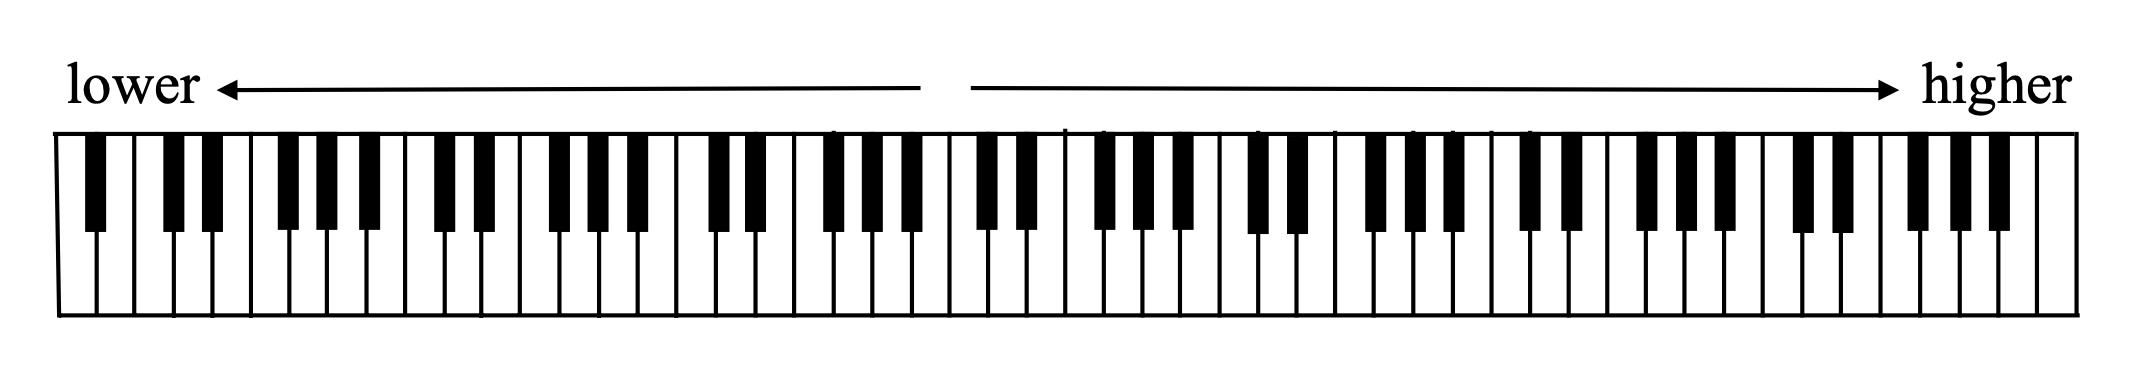
\includegraphics[width=\textwidth]{assets/piano}
    \caption{~A piano with 88 keys and indicated pitches~\cite{music-theory}}\label{fig:piano}
\end{figure}


\section{Notation}\label{sec:notation}

Notes are written on a five-line \textit{staff} (figure~\ref{fig:staff}).
A \textit{clef} orients the lines to a reference point.
For example, when placed on a five-line staff, the \textit{G clef} becomes the \textit{treble clef}, the most well-known \textit{clef}.
In treble clef, the notes on the lines are E--G--B--D--F from lowest to highest, often remembered through the traditional mnemonic\footnote{Every Good Boy Does Fine}.
The spaces are F--A--C--E from lowest to highest.
\textit{Staves} (the plural of ``staff'') are extended by the ledger lines (figure~\ref{fig:staff}).~\cite{music-theory}


\begin{figure}
    \centering
    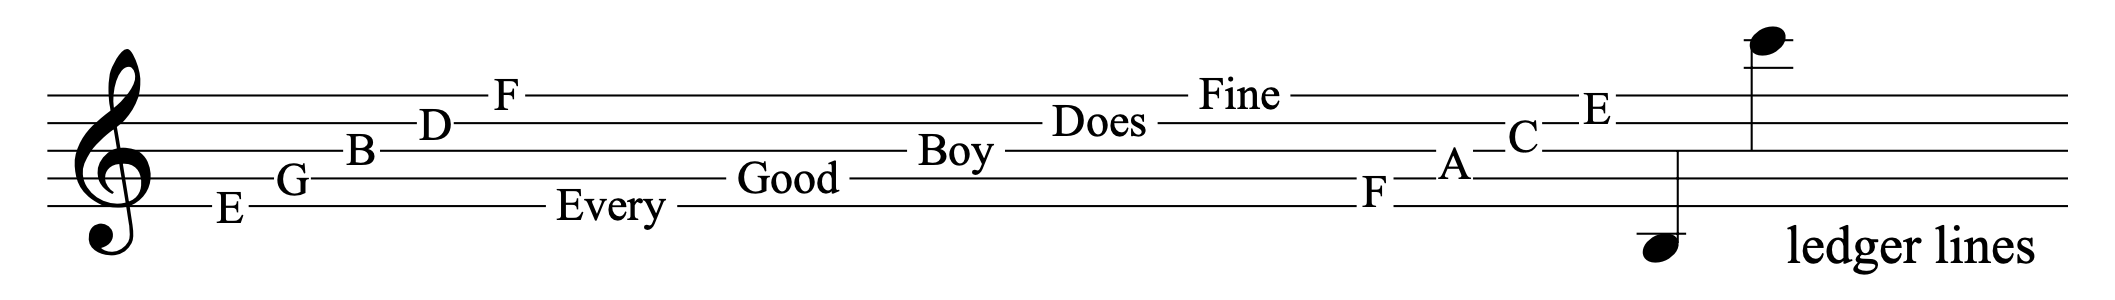
\includegraphics[width=\textwidth]{assets/staff}
    \caption{~The staff with a treble clef~\cite{music-theory}}\label{fig:staff}
\end{figure}


\section{Octave registers}\label{sec:octave-registers}

The note names used in music are \textit{ABCDEFG} (known as the ``musical alphabet'').
After G, note A returns, and \textit{ABCDEFG} occurs again.
An octave is a distance from any note to the same note in the next or previous register.
A piano also contains so-called \textit{accidentals} (special keys that raise or lower a note's pitch).
The piano keyboard with 88 notes consists of seven octaves (composed of seven notes and five accidentals) along with three extra notes and one extra accidental.~\cite{music-theory}

When learning about octave registers, we focus on note C for reasons that will soon become clear after learning about the major scale.
We use octave registers (C4, D5, \ldots) to specify the note's exact register.
The note C4 is known as \textbf{``middle C''} and is a vital reference point.
See the keyboard in the figure~\ref{fig:octave-registers}.~\cite{music-theory}

\begin{figure}
    \centering
    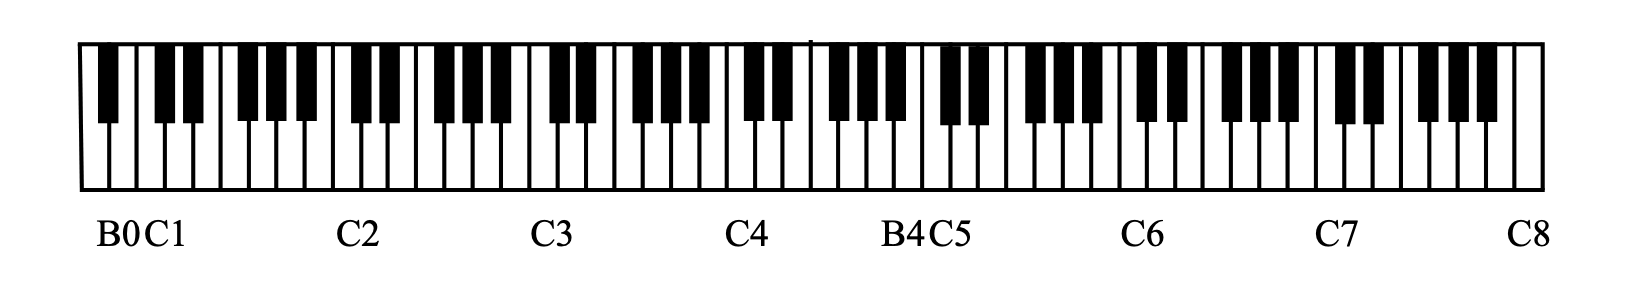
\includegraphics[width=\textwidth]{assets/octave-registers}
    \caption{~A piano with octave registers denoted~\cite{music-theory}}\label{fig:octave-registers}
\end{figure}

Notice that the register number changes after note B each time (e.g., B4 is followed by C5).
In the treble clef notation, middle C is placed on the \textit{ledger line} below the staff.
In the bass clef, the \textit{middle C} is placed on the \textit{ledger line} above the staff.
Both notations are visible in figure~\ref{fig:middle-c}.~\cite{music-theory}

\begin{figure}
    \centering
    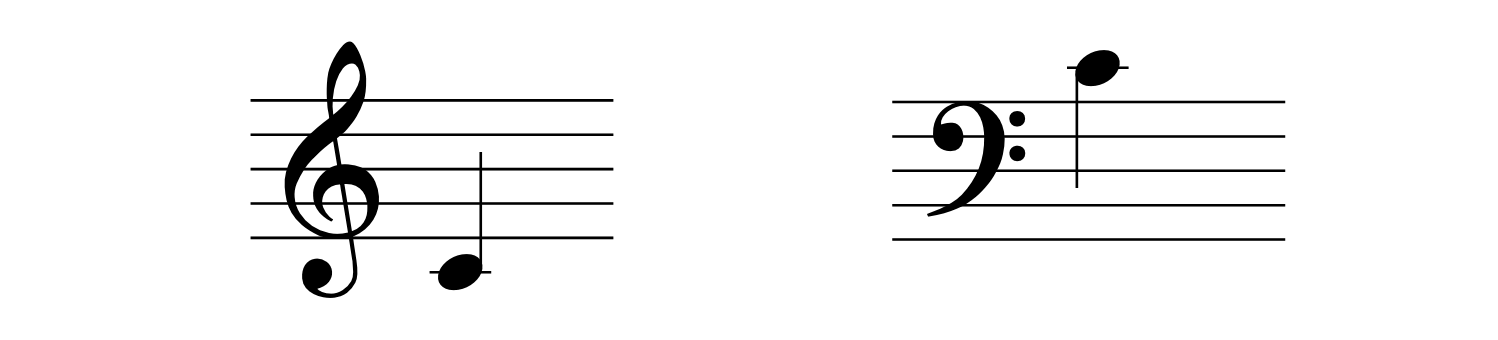
\includegraphics[width=\textwidth]{assets/middle-c}
    \caption{~Middle C (C4) in treble clef and bass clef~\cite{music-theory}}\label{fig:middle-c}
\end{figure}

When we join the treble and the bass clef together by a bracket, we create the so-called \textbf{grand staff}, how piano music is written.
An example of the \textbf{grand staff} is shown in figure~\ref{fig:grand-staff}.~\cite{music-theory}


\begin{figure}
    \centering
    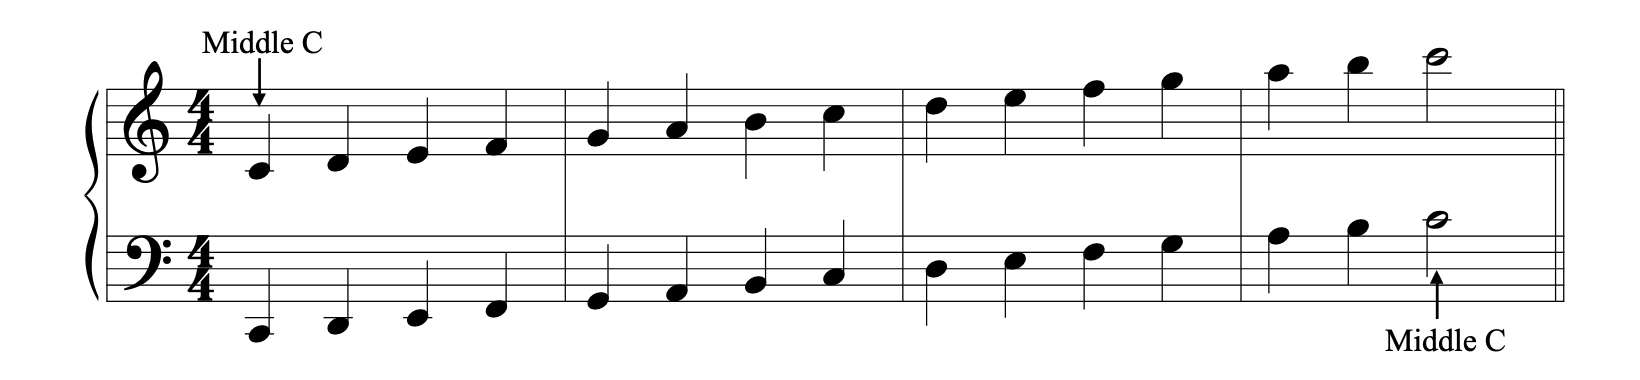
\includegraphics[width=\textwidth]{assets/grand-staff}
    \caption{~The grand staff~\cite{music-theory}}\label{fig:grand-staff}
\end{figure}


\section{Accidentals}\label{sec:accidentals}

Accidentals are characters that we use to modify the following note (either raise or lower the note pitch).
The following five symbols exist~\cite{music-theory}:

\begin{itemize}
    \item \textit{Sharp} symbol (\sh) raises pitch half a step
    \item \textit{Flat} symbol (\fl) lowers pitch half a step
    \item Double \textit{sharp} symbol (\musDoubleSharp) raises pitch two halves a step (a whole step)
    \item Double \textit{flat} symbol (\musDoubleFlat) lowers pitch two halves a step (a whole step)
    \item \textit{Natural} symbol (\na) cancels out accidentals previously applied in a measure of Major Key Signatures or Minor Key Signatures
\end{itemize}


\section{Half Steps and Whole Steps}\label{sec:half-whole-steps}

A half step on a piano keyboard is the distance from one note to the following immediate note.
A whole step composes of two half steps (figure~\ref{fig:half-whole-steps}).~\cite{music-theory}


\begin{figure}
    \centering
    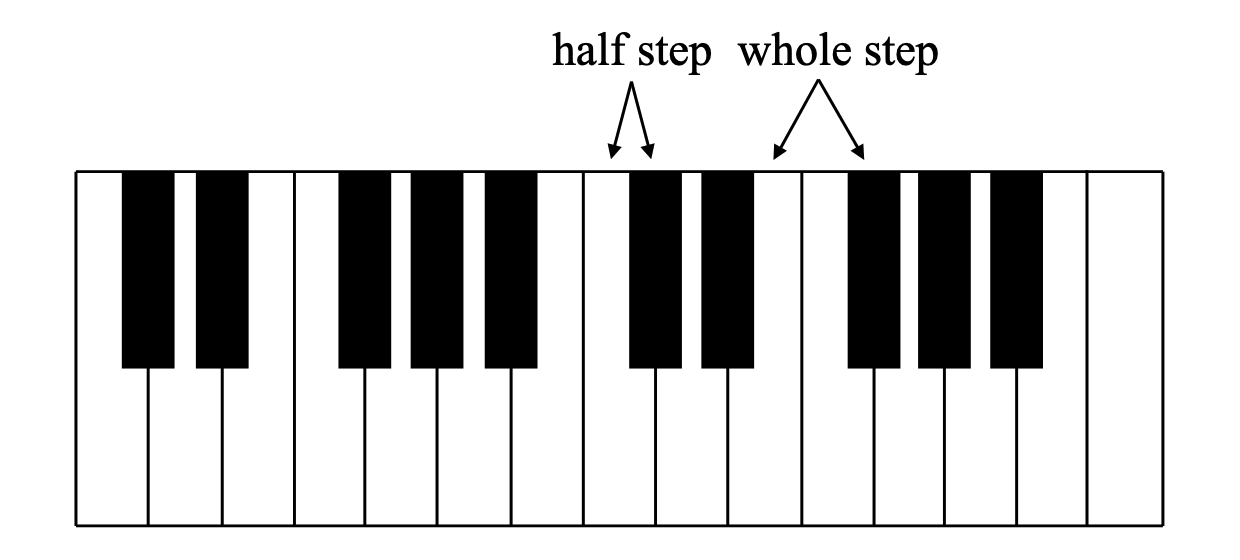
\includegraphics[width=0.78\textwidth]{assets/half-whole-steps}
    \caption{~The half step and whole step~\cite{music-theory}}\label{fig:half-whole-steps}
\end{figure}


\section{The Major scale}\label{sec:major-scale}

A specific sequence of whole and half steps is called a \textit{major scale}.
It is helpful to think of the pattern as consisting of two \textit{tetrachords}\footnote{\textit{``a tetrachord is a four-note scale segment''~\cite{music-theory}}} and a single whole step.
The lower \textit{tetrachord} is of the following pattern: whole step, whole step, half step.
A whole step then joins both \textit{tetrachords} together.
The upper \textit{tetrachord} consists of the same pattern as the lower one: whole step, whole step, half step.
If we use W for the whole step and H for the half step, we can write the major scale pattern as W--W--H, Whole–step connection, W--W--H.~\cite{music-theory}


\begin{figure}
    \centering
    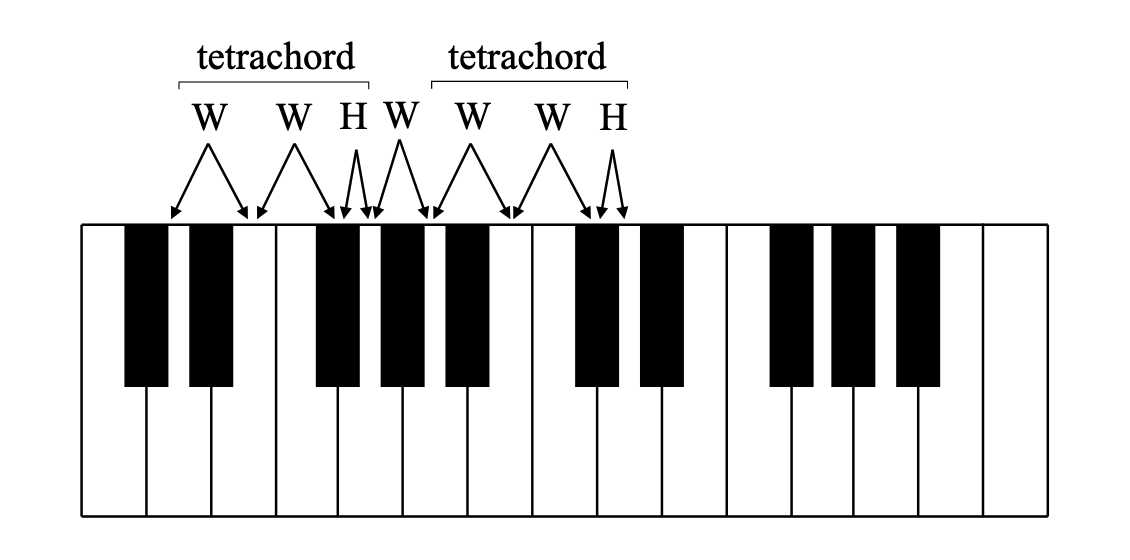
\includegraphics[width=0.8\textwidth]{assets/major-scale-keyboard}
    \caption{~The D major scale on a keyboard~\cite{music-theory}}\label{fig:major-scale-keyboard}
\end{figure}


\begin{figure}
    \centering
    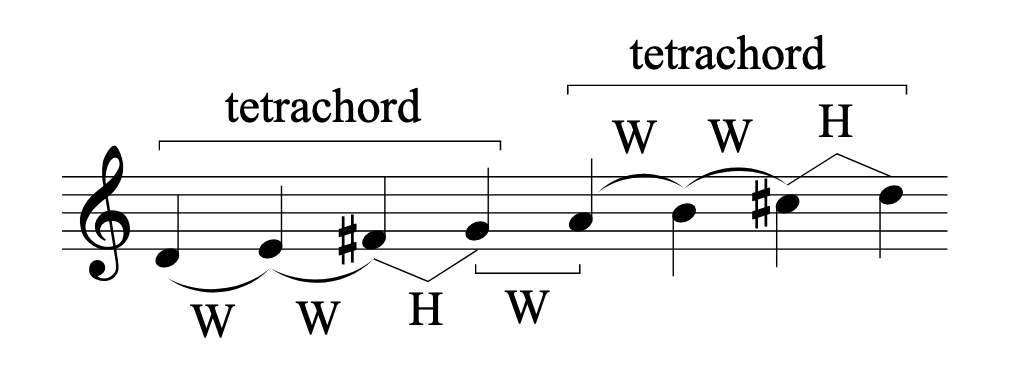
\includegraphics[width=0.84\textwidth]{assets/major-scale-staff}
    \caption{~The D major scale in treble clef~\cite{music-theory}}\label{fig:major-scale-staff}
\end{figure}

Note that all \textit{major scales} use the notes of the musical alphabet in order;
no notes get skipped, and no note occurs twice.
In figure~\ref{fig:major-scale-staff}, the first four notes are D--E--F\textsuperscript{\sh}--G, not D--E--G\textsuperscript{\fl}--G.
In D--E--G\textsuperscript{\fl}--G, G incorrectly occurs twice, and the F\textsuperscript{\sh} between E and G gets skipped.~\cite{music-theory}


\section{Major key signatures}\label{sec:major-key-signatures}

The key signature is a notation positioned next to the clef at the beginning of a piece or section.
We use it to hint which sharps or flats are in the piece's scale to prevent the composer from writing every sharp/flat from the scale each time it occurs.~\cite{music-theory}

There are \textbf{15} major \textit{key signatures}.
The key of \textit{C major has no sharps or flats} in the key signature, while the other key signatures can have between \textit{1 to 7 sharps} and \textit{1 to 7 flats}, resulting in the other 14 key signatures.
Notations of the major key signatures can be seen in figures 23 and 24 for sharps and flats, respectively.~\cite{music-theory}


\begin{figure}
    \centering
    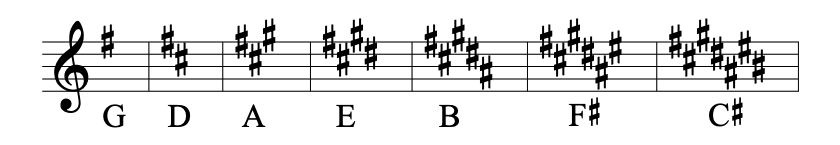
\includegraphics[width=\textwidth]{assets/major-signatures-sharps}
    \caption{~Major key signatures in sharps~\cite{music-theory}}\label{fig:major-signatures-sharps}
\end{figure}


\begin{figure}
    \centering
    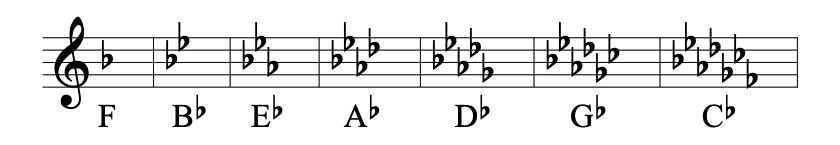
\includegraphics[width=\textwidth]{assets/major-signatures-flats}
    \caption{~Major key signatures in flats~\cite{music-theory}}\label{fig:major-signatures-flats}
\end{figure}

\textit{``A helpful learning device to remember the order of keys in relation to the order of sharps and flats is the \textbf{circle of fifths}.
As you ascend in fifths (clockwise), key signatures get one degree `sharper.'
    (C to G is a fifth because C=1, D=2, E=3, F=4, and G=5.)
    As you descend in fifths (counterclockwise), key signatures get one degree `flatter.'{''}}~\cite{music-theory}~(figure~\ref{fig:circle-of-fifths})


\begin{figure}
    \centering
    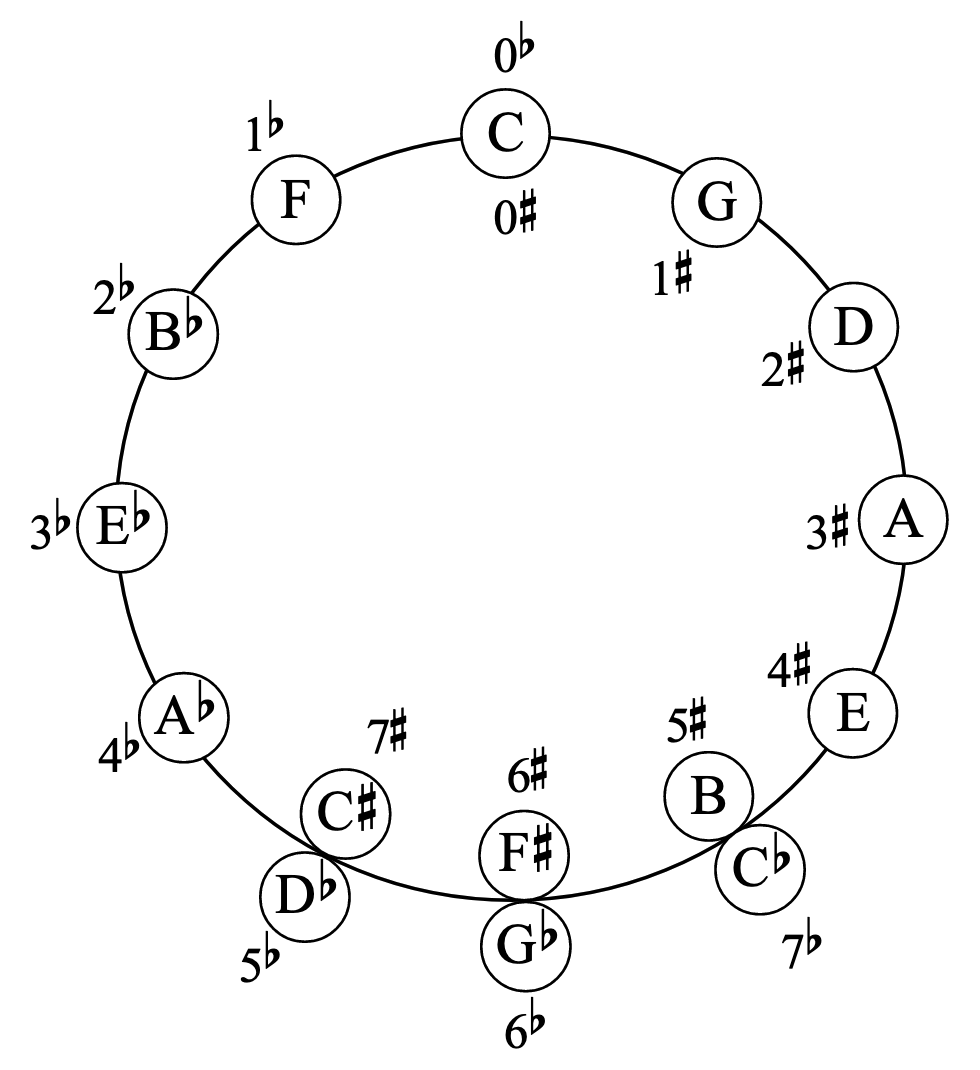
\includegraphics[width=0.6\textwidth]{assets/circle-of-fifths}
    \caption{~Circle of fifths in major keys~\cite{music-theory}}\label{fig:circle-of-fifths}
\end{figure}

Notice the overlapping keys at the bottom of the circle.
B major is enharmonically\footnote{pitches that are the same notes on a piano but are written differently on the staff} the same as C\textsuperscript{\fl} major, F\textsuperscript{\sh} major is enharmonically the same as G\textsuperscript{\fl} major, and C\textsuperscript{\sh} major is enharmonically the same as D\textsuperscript{\fl} major.~\cite{music-theory}


\section{Minor scales}\label{sec:minor-scales}

Alongside the \textit{major scale}, there are also three \textit{minor scales}: the \textit{natural minor scale}, the \textit{harmonic minor scale}, and the \textit{melodic minor scale}.
The \textit{melodic minor scale} has an ascending version, and a descending version that is the same as the \textit{natural minor scale}.
Both can be seen in figure~\ref{fig:minor-scale}.


\begin{figure}
    \centering
    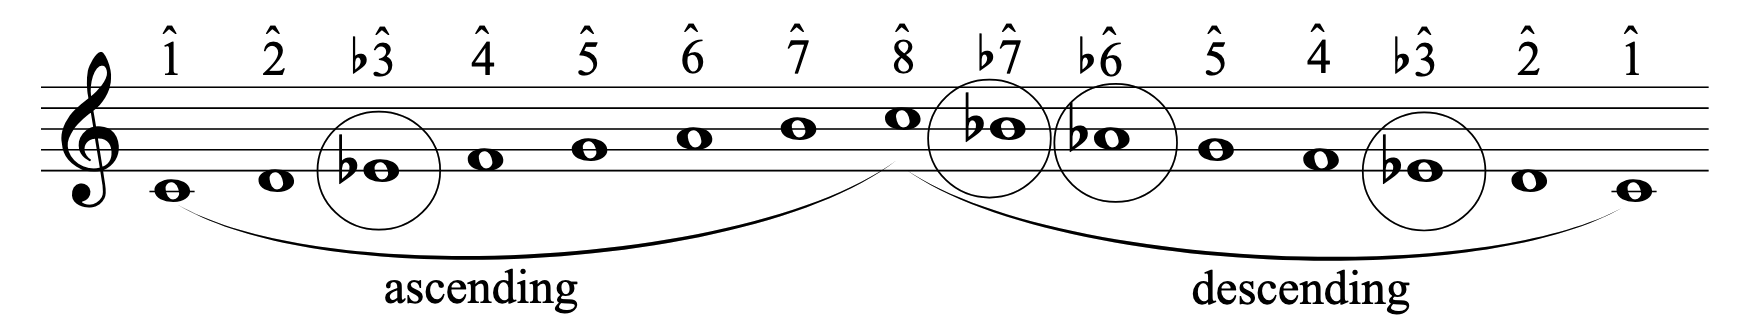
\includegraphics[width=\textwidth]{assets/minor-scale}
    \caption{~Melodic minor scale~\cite{music-theory}}\label{fig:minor-scale}
\end{figure}


\section{Minor key signatures}\label{sec:minor-key-signatures}

\textit{Minor key signatures} agree with the notes of the natural minor scale.
Since the C natural minor scale had E\textsuperscript{\fl}, A\textsuperscript{\fl} and B\textsuperscript{\fl} accidentals, the key signature of C minor has three flats, written in the order of flats (B\textsuperscript{\fl}, E\textsuperscript{\fl}, A\textsuperscript{\fl}).~\cite{music-theory}


\begin{figure}
    \centering
    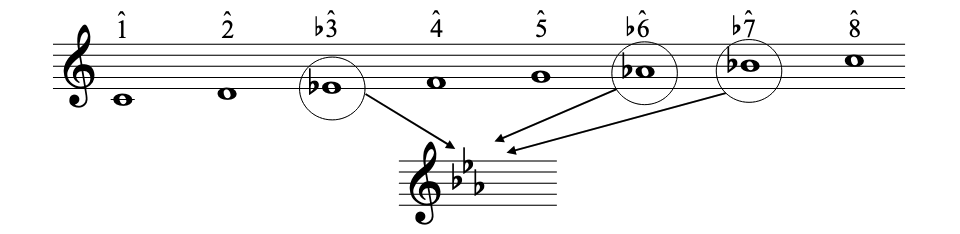
\includegraphics[width=\textwidth]{assets/natural-in-major}
    \caption{~Natural minor scale in major key signature~\cite{music-theory}}\label{fig:natural-in-major}
\end{figure}


\begin{figure}
    \centering
    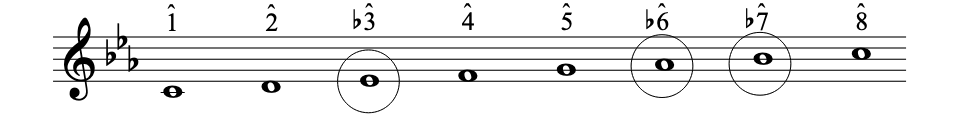
\includegraphics[width=\textwidth]{assets/natural-in-minor}
    \caption{~Natural minor scale in minor key signature~\cite{music-theory}}\label{fig:natural-in-minor}
\end{figure}


A \textit{minor key signature} will have three lowered notes—the third, sixth and seventh—related to the corresponding major key signature.
We use the term \textit{parallel minor} when referring to a minor scale (e.g., the parallel major of F minor is F major) with the same first scale degree (in this case C) as the major.
One method of figuring out a minor key signature is to add three flats (or subtract three sharps) to the parallel major key signature.
When writing below the five-line staff to designate keys, we use upper case for major keys and \textit{lowercase for minor keys}.
~\cite{music-theory}


\begin{figure}
    \centering
    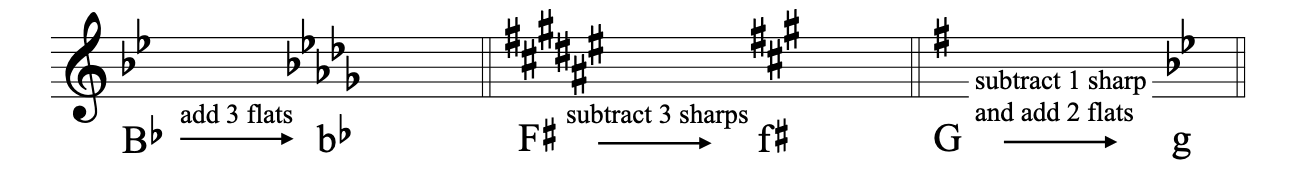
\includegraphics[width=\textwidth]{assets/parallel-minors}
    \caption{~Parallel minor keys signatures~\cite{music-theory}}\label{fig:parallel-minors}
\end{figure}

We also add figures of minor key signatures (figure~\ref{fig:minor-key-signatures}) and circle of fifths (figure~\ref{fig:circle-of-fifths-minor}) for minor scale for completeness.


\begin{figure}
    \centering
    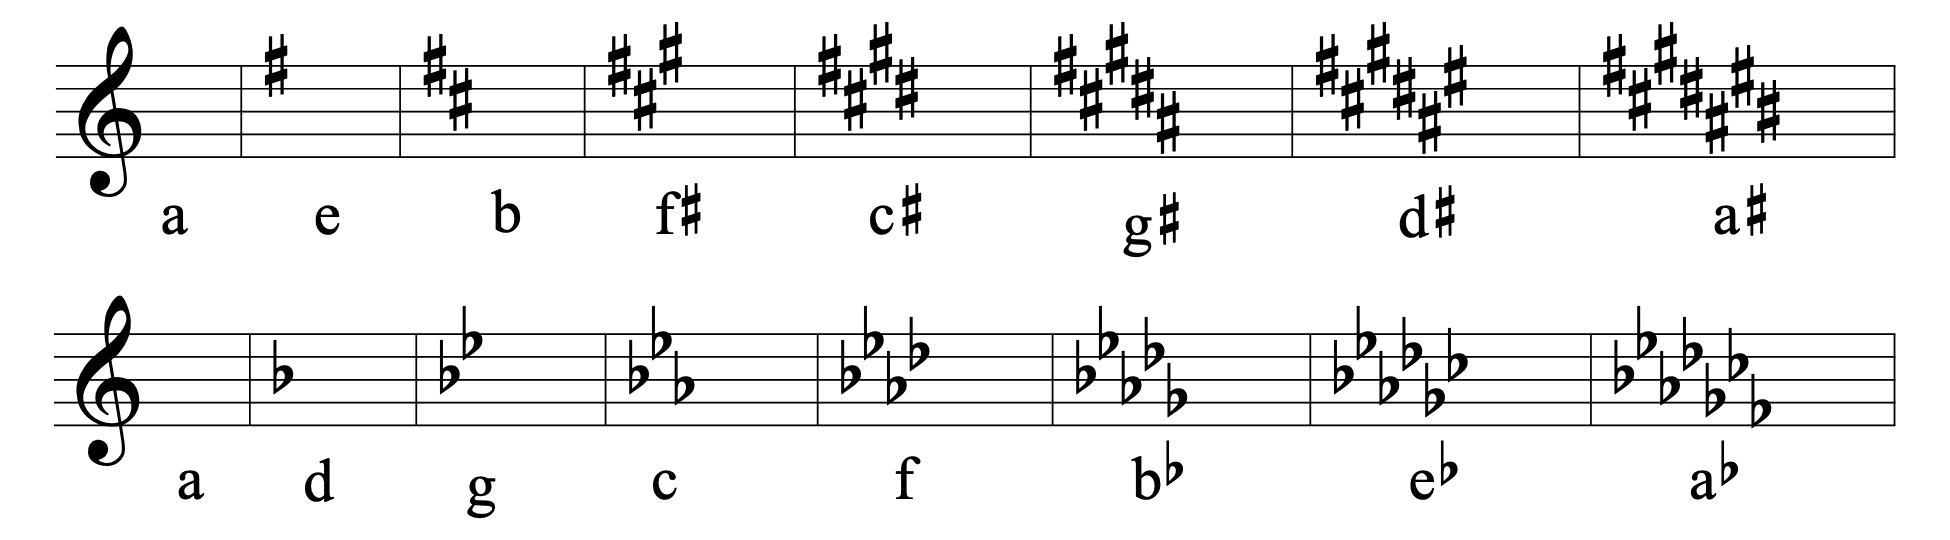
\includegraphics[width=\textwidth]{assets/minor-key-signatures}
    \caption{~Minor keys signatures~\cite{music-theory}}\label{fig:minor-key-signatures}
\end{figure}



\begin{figure}
    \centering
    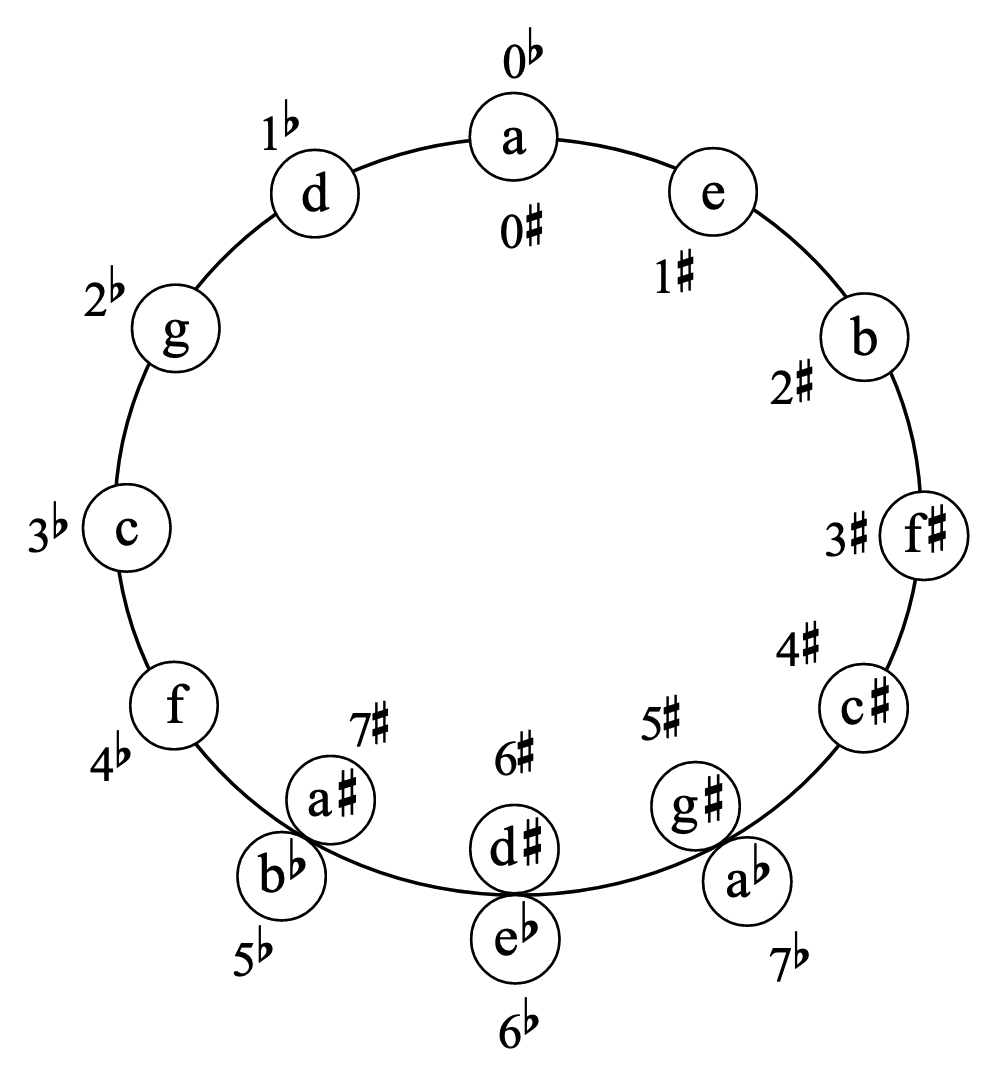
\includegraphics[width=0.6\textwidth]{assets/circle-of-fifths-minor}
    \caption{~Circle of fifths in minor keys~\cite{music-theory}}\label{fig:circle-of-fifths-minor}
\end{figure}


\section{Time signature}\label{sec:time-signature}


The staff can also contain a \textit{time signature} next to a clef.
We denote it as two stacked numbers;
the lower number is typically a number corresponding to a power of 2 and tells us the relative duration of a note, while the upper number hints at how many pulses (or \textit{beats}) we can expect per \textit{bar}\footnote{specified segment of time corresponding to the number of beats}.~\cite{music-theory}


\begin{figure}
    \centering
    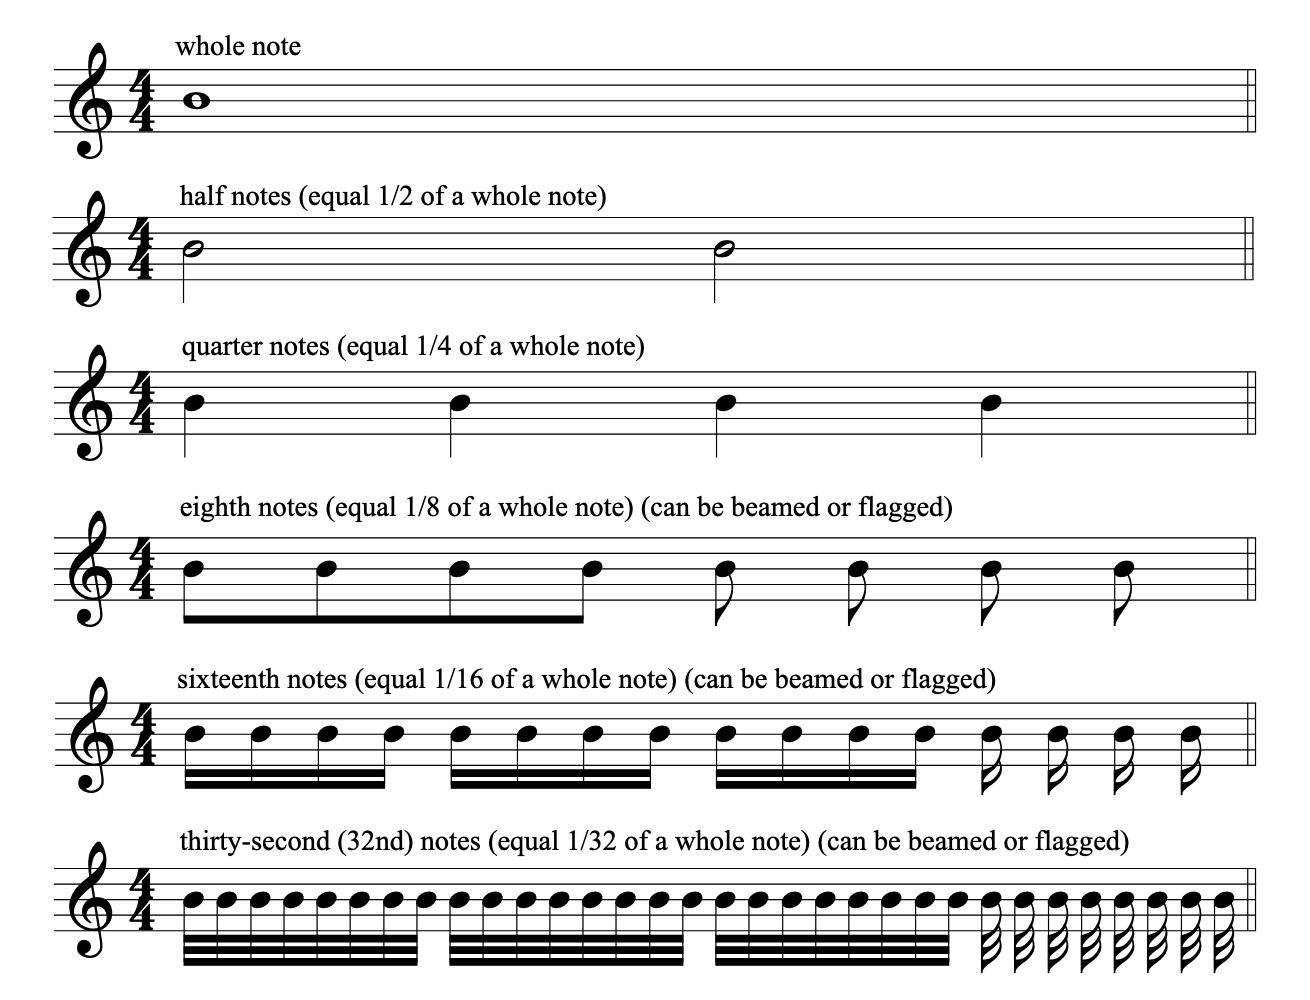
\includegraphics[width=0.8\textwidth]{assets/common-time-notes}
    \caption{~Different notes used for a common time~\cite{music-theory}}\label{fig:common-time-notes}
\end{figure}


\section{Durational symbols}\label{sec:durational-symbols}

The most common \textit{time signature} is $_{4}^{4}$ (also known as ``common time'').
It makes sense to introduce \textit{durational symbols} in the context of $_{4}^{4}$ time signature because a whole note takes up a full measure in $_{4}^{4}$, a half note takes up half a measure of $_{4}^{4}$, a quarter note takes up $\frac{1}{4}$ of a measure, and so on.


\begin{figure}
    \centering
    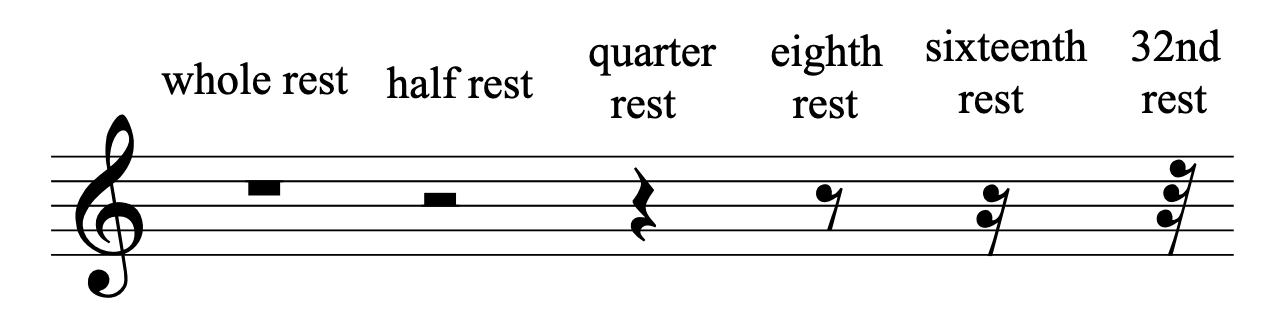
\includegraphics[width=0.9\textwidth]{assets/durational-symbols}
    \caption{~Durational symbols for rests~\cite{music-theory}}\label{fig:durational-symbols}
\end{figure}

Meter describes the number of beats in a measure (also called a bar) and how we typically divide the beats.
A beat is a basic pulse measured in music and thus the unit in which we think about music.
Pulse and beat are interchangeable.
The speed of a beat is called tempo.
We can state tempo in beats per minute (\textit{bpm}), such as 60bpm (where the rate of the beat would be equal to a second), or, in classical music, with terms like Allegro, Andante, and Adagio, sometimes in combinations with ``M.M.'' for Maelzel's Metronome.~\cite{music-theory}

Some meters have a special name;
meters with two beats in a bar are called \textit{duple}, three beats in a bar \textit{triple}, and four beats in a bar \textit{quadruple}.
Meter is described as \textit{simple} if the beats are normally divided into two parts and \textit{compound} if the beats are normally divided into three parts.~\cite{music-theory}

